\section{Anexo A: esquema inicial a mano}

\begin{figure}[H]
  \centering
  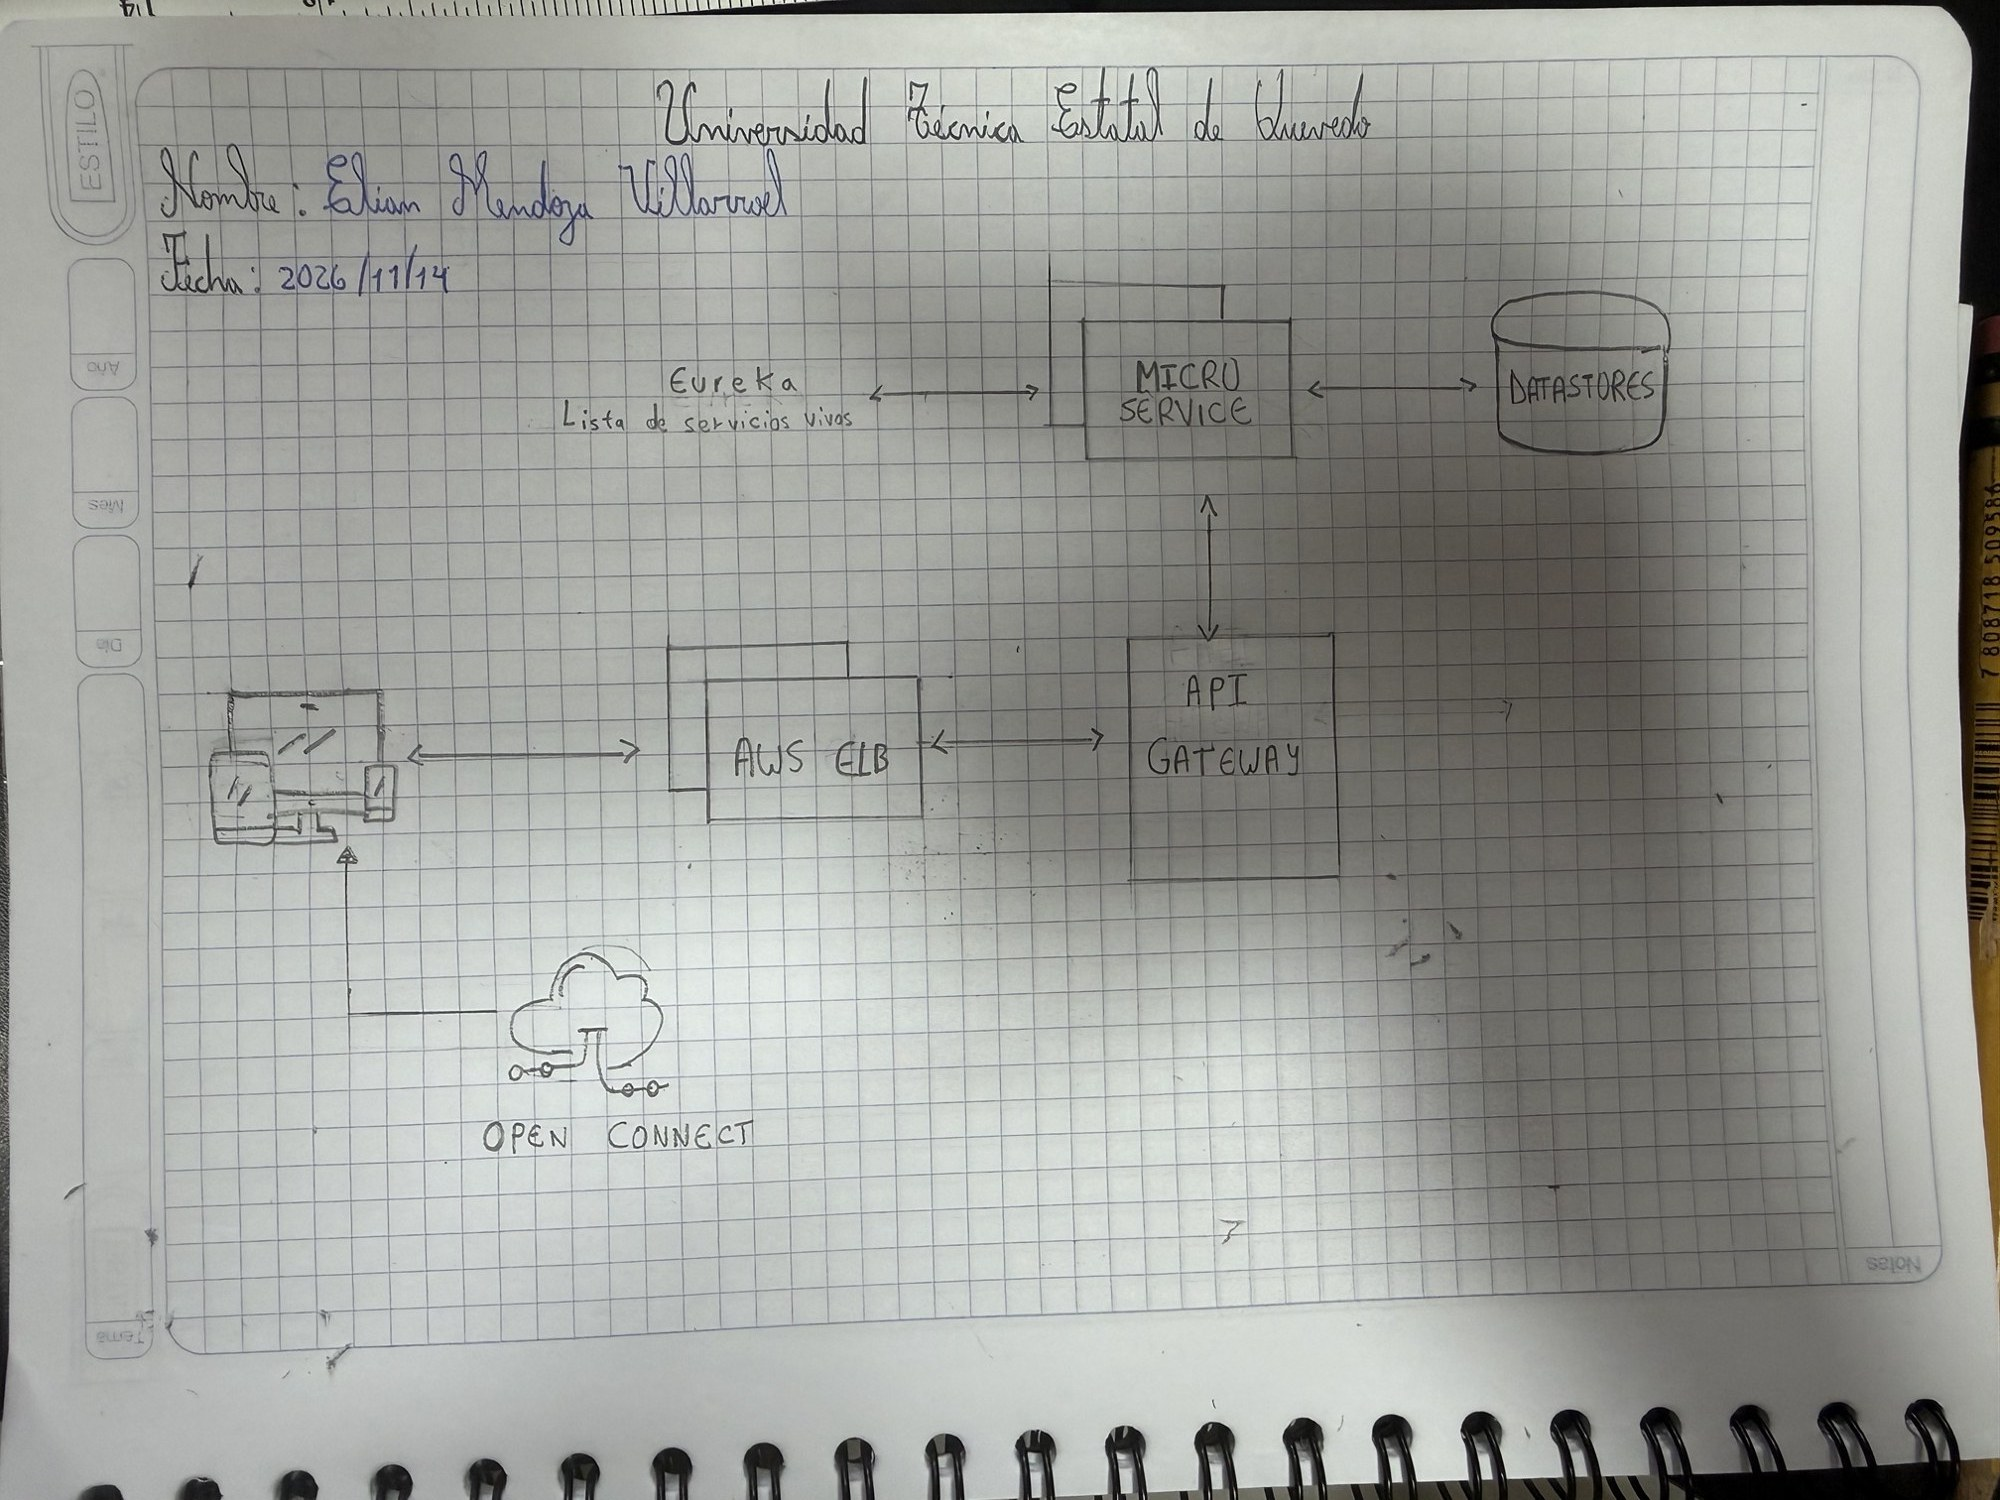
\includegraphics[width=\textwidth]{anexo-a-esquema-mano.jpg}
  \caption{Primer bosquejo de la arquitectura de Netflix, dibujado a mano por el autor (14 de noviembre de 2026).}
  \label{fig:anexoA}
\end{figure}

\section{Anexo B: capturas de lectura de las fuentes}

\begin{figure}[H]
  \centering
  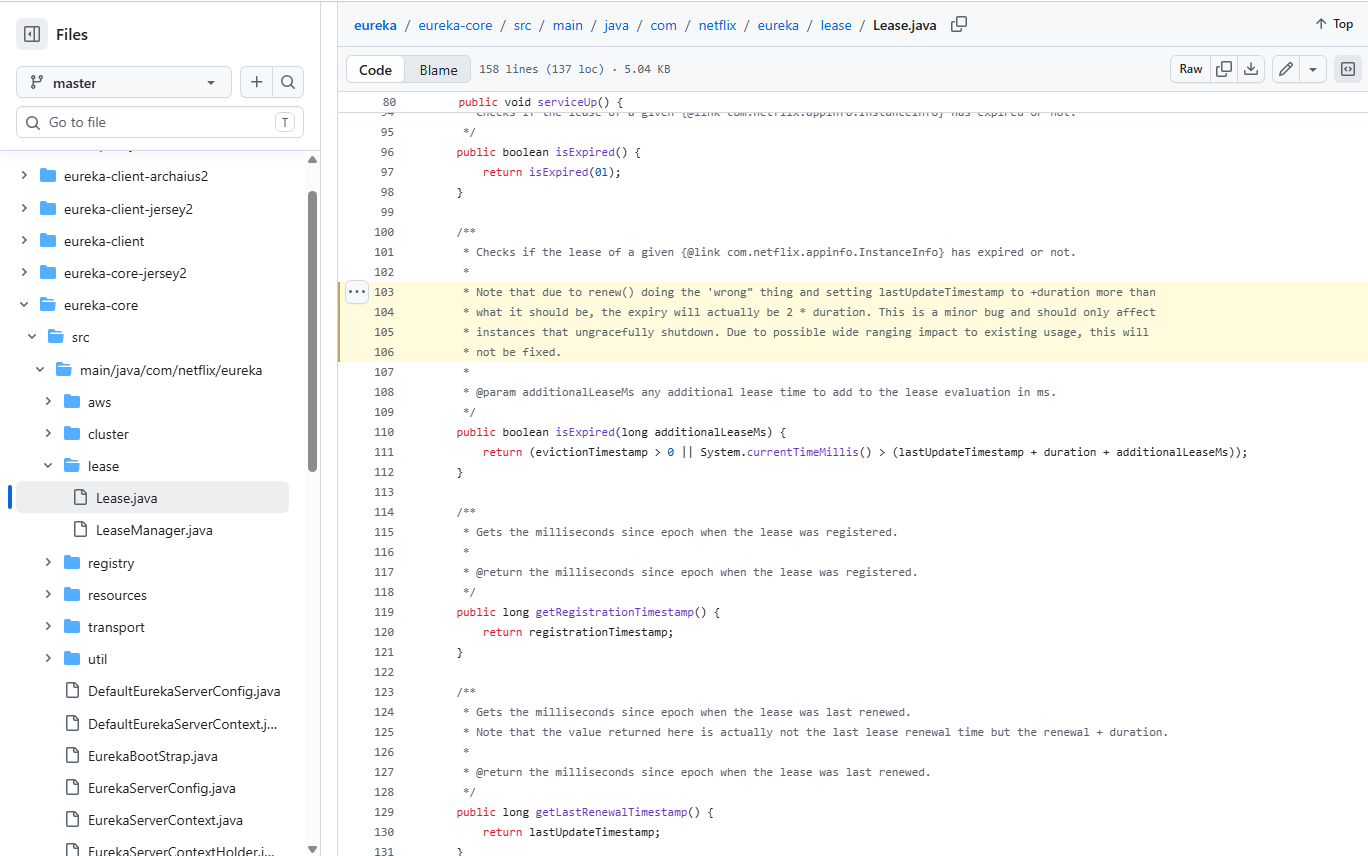
\includegraphics[width=\textwidth]{anexo-b-1.png}
  \caption{Código fuente de Eureka, archivo \texttt{Lease.java}, líneas 103 a 106~\cite{Eureka_Lease}. Citado en la sección Experimentación propia para explicar por qué Eureka tardó 30 segundos y no 15.}
  \label{fig:anexoB1}
\end{figure}

\begin{figure}[H]
  \centering
  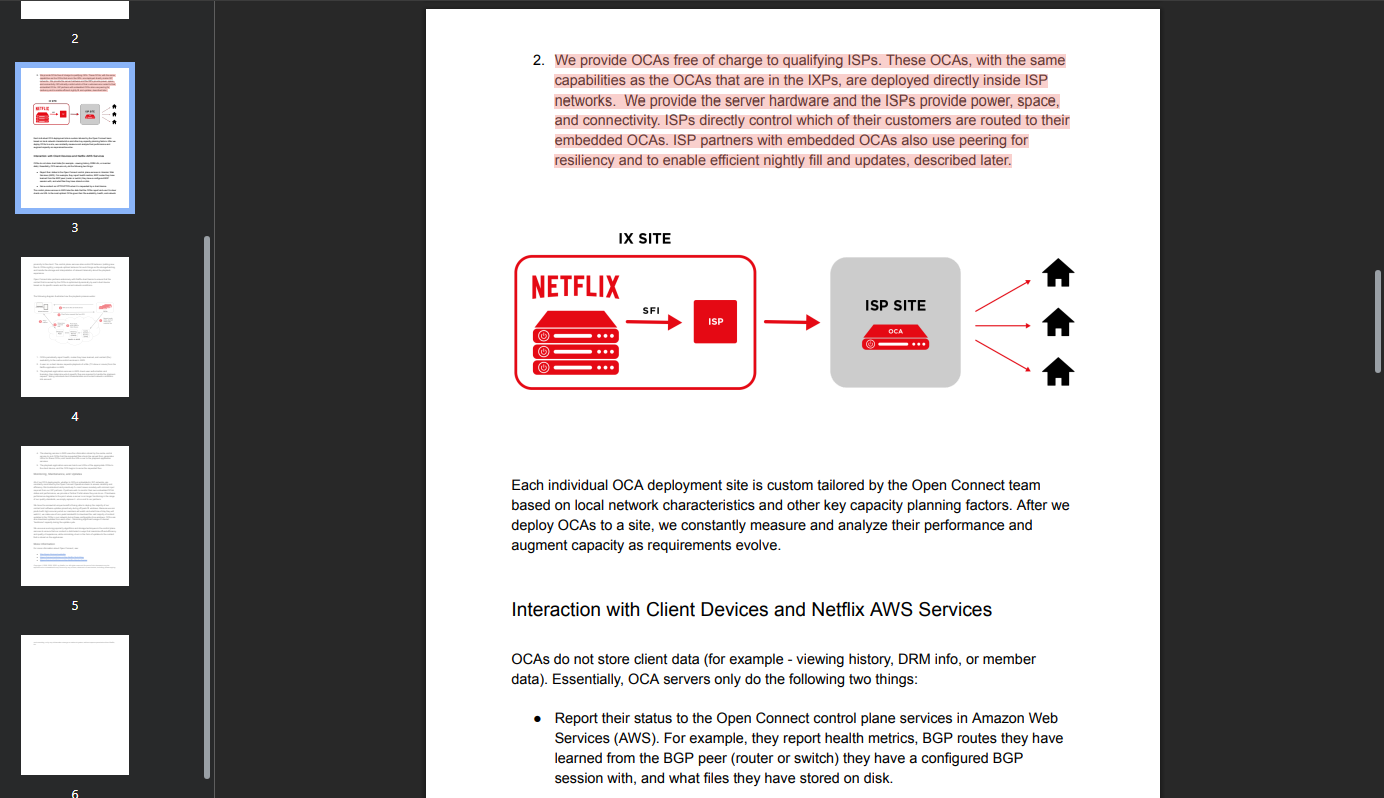
\includegraphics[width=\textwidth]{anexo-b-2.png}
  \caption{\textit{Open Connect Overview}, p.~3~\cite{Netflix_OpenConnect}. Citado en la Introducción y en la Arquitectura del sistema: los servidores de Open Connect se instalan dentro de los proveedores de internet.}
  \label{fig:anexoB2}
\end{figure}

\begin{figure}[H]
  \centering
  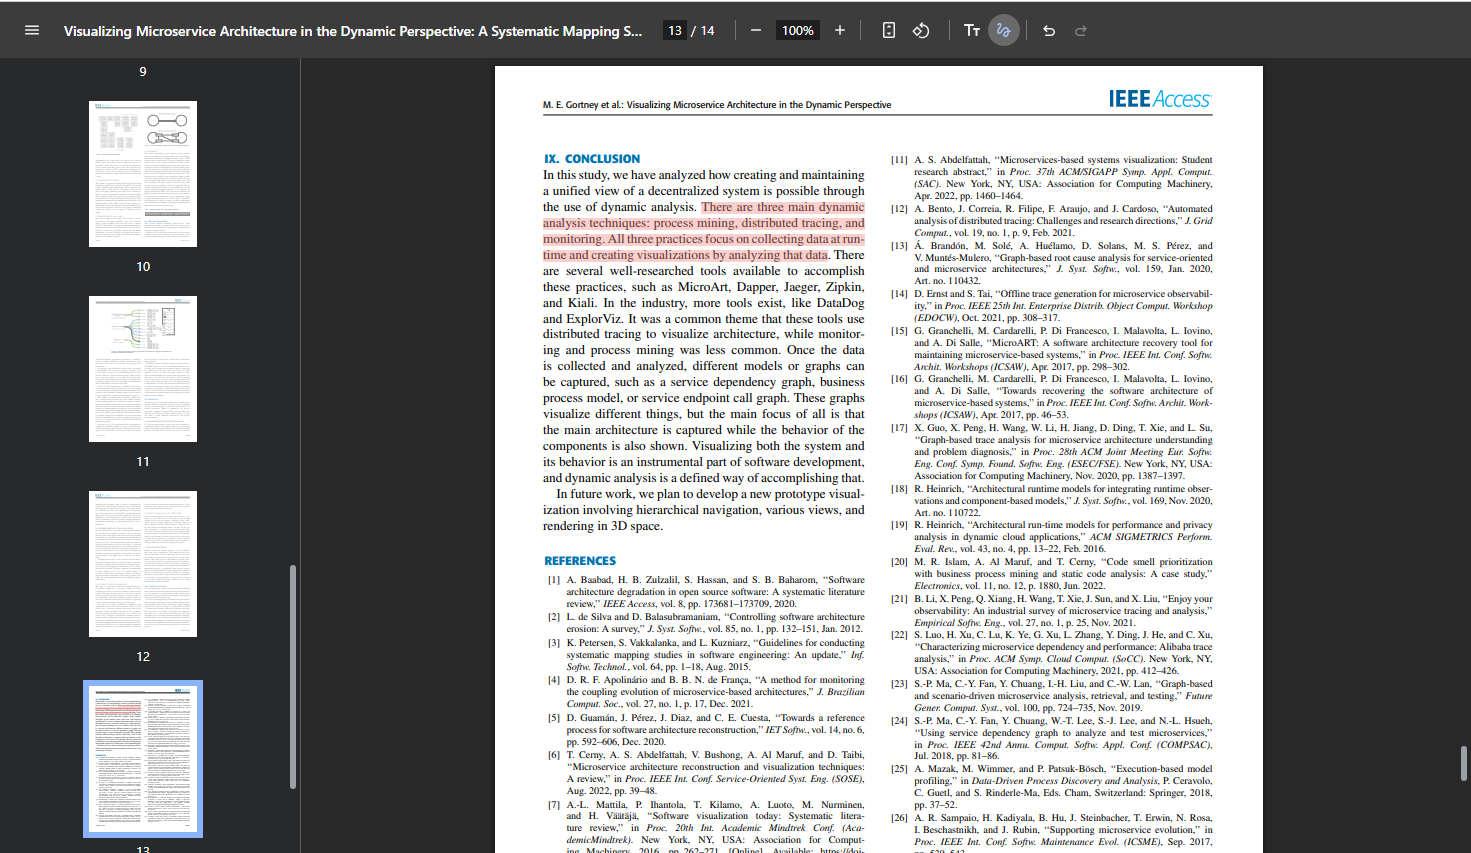
\includegraphics[width=\textwidth]{anexo-b-3.png}
  \caption{Gortney \textit{et al.}, p.~120011~\cite{Gortney_2022}. Citado en la Postura crítica: rastrear errores entre muchos servicios requiere técnicas como el rastreo distribuido y la monitorización.}
  \label{fig:anexoB3}
\end{figure}
